\section{Pre-processing Techniques for \ltlf Synthesis}
In this section, we introduce three pre-processing techniques for \ltlf synthesis, which can be evaluated immediately on the given \ltlf formula w.r.t. the atomic set $\P=\X\cup\Y$. First, the following Lemma is straightforward according to the \ltlf semantics and Definition \ref{def:synthesis}.

\begin{theorem}\label{thm:sat-syn}
	If the \ltlf formula $\phi$ is unsatisfiable, then $\phi$ is unrealizable; If $\phi$ is valid, then $\phi$ is realizable.
\end{theorem}
Theorem~\ref{thm:sat-syn} suggests that an unsatisfiable/valid \ltlf formula is not quite useful as a synthesis specification in practice. 
To that end, an extant \ltlf-satisfiability solver, e.g., \aaltaf~\cite{LRPZV19}, can be used to check the satisfiability/validity of the formula before synthesis. We now define the $\satOnce$ predicate for further use. 

\begin{definition}\label{def:satOnce}
Given an \ltlf formula $\phi$ and $\omega \in 2^{\P}$, we define the predicate $\satOnce (\omega, \phi)$ is true iff 
\begin{itemize}
	\item $\phi$ is $\tt$; or
	\item $\phi$ is an atom and $\phi \in \omega$; or 
	\item $\phi = \neg\psi$ and $\neg \satOnce (\omega, \psi)$ is true; or
	\item $\phi = \phi_1\wedge\phi_2$ and $\satOnce (\omega, \phi_1)$ and $\satOnce (\omega, \phi_2)$ are true; or
	\item $\phi = \phi_1\vee\phi_2$ and $\satOnce (\omega, \phi_1)$ or $\satOnce (\omega, \phi_2)$ is true; or
	\item $\phi = \phi_1\U\phi_2$ or $\phi = \phi_1\R\phi_2$ and $\satOnce (\omega, \phi_2)$ is true.
\end{itemize} 
\end{definition}

Notably, $\satOnce (\omega, \ocircle\psi)$ can never be true, while $\satOnce (\omega, \N\psi)$ is always true. Based on Definition \ref{def:satOnce} and the semantics of \ltlf formulas, the lemma below is straightforward. 

\begin{lemma}\label{lem:satOnce}
Given an \ltlf formula $\phi$ and $\omega\in 2^{\P}$, $\satOnce (\omega, \phi)$ is true iff $\omega\models\phi$ holds.
\end{lemma}
In fact, Definition \ref{def:satOnce} can be considered as the simplified version of \ltlf semantics in which the length of the finite trace is restricted to be one. Definition \ref{def:satOnce} is provided as a better option for the implementation purpose. 

\begin{theorem}\label{thm:winning-1}
Given an \ltlf formula $\phi$ with alphabet $\X\cup \Y$, if there exists $Y\in 2^{\Y}$ such that $\satOnce (Y, \phi)$ is true, then $\phi$ is realizable. 
\end{theorem}
\begin{proof}
From Lemma \ref{lem:satOnce}, $\satOnce (Y, \phi)$ is true implies that $Y\models\phi$ is true. As a result, for every $X\in 2^{\X}$, $X\cup Y\models\phi$ is true, providing that $\X\cap \Y=\emptyset$. Therefore, there exists a strategy $g$ with $g(\epsilon) = Y$ such that for every $X\in 2^{\X}$ it holds that $X\cup g(\epsilon)\models\phi$. According to Definition \ref{def:synthesis}, $g$ is a winning strategy for the system and $\phi$ is realizable.
\end{proof}

Consider the formula $a\U b$ with $\X=\{a\}$ and $\Y=\{b\}$ as an example. Let $Y= \{b\}$ and since $\satOnce (Y, a\U b)$ is true, $\phi$ is realizable according to Theorem~\ref{thm:winning-1}. It is easy to induce that Theorem~\ref{thm:winning-1} can be extremely helpful for the synthesis instances like $\psi\U b$ with $\Y=\{b\}$, under which the realizable result can be achieved by Theorem~\ref{thm:winning-1} directly without further automata construction. This advantage may potentially lead to an exponential better performance, which will be discussed in the experimental section later. Next, we introduce the concept of \emph{formula projection} for the pre-processing of unrealizable formulas. 

\begin{definition}[Formula Projection]\label{def:fp}
Given an \ltlf formula $\phi$ in \NNF with the atomic set $\P$, we define its projection under $\P$, denoted as $\phi |_\P$, is a Boolean formula as follows:
\begin{itemize}
	\item $\phi|_\P = \phi$ if $\phi$ is $\tt$, $\ff$ or a literal;
	\item $\phi|_\P = \tt$ if $\phi = \ocircle\psi$ or $\phi = \N\psi$;
	\item $\phi|_\P = \phi_1|_\P \wedge \phi_2|_\P$ if $\phi = \phi_1\wedge\phi_2$;
	\item $\phi|_\P = \phi_1|_\P \vee \phi_2|_\P$ if $\phi = \phi_1\vee\phi_2$;
	\item $\phi|_\P = \phi_1|_\P \vee \phi_2|_\P$ if $\phi = \phi_1\U\phi_2$;
	\item $\phi|_\P = \phi_2|_\P$ if $\phi = \phi_1\R\phi_2$.
\end{itemize}
\end{definition}

\begin{lemma}\label{lem:fp}
Given an \ltlf formula $\phi$ and a finite trace $\eta$, $\eta\models\phi$ implies that $\eta[0]\models\phi|_\P$.
\end{lemma}
The proof can be done by induction over the structure of $\phi$, which is omitted here. Lemma \ref{lem:fp} indicates that $\phi|_\P$ is sufficient to capture all the first-position elements of $\phi$'s accepting traces. Inspired by that, we have the following theorem that can help with identifying a formula being unrealizable. 

\begin{theorem}\label{thm:failure-1}
Given an \ltlf formula $\phi$ with the atomic set $\X\cup \Y$, if there does not exists $Y\in 2^{\Y}$ such that $Y\models \phi|_{\X\cup\Y}$, then $\phi$ is unrealizable. 
\end{theorem}
\begin{proof}
Assume $\phi$ is realizable. According to Definition \ref{def:synthesis}, there exists a winning strategy $g$ such that for an arbitrary infinite sequence $X_0,X_1,\ldots\in (2^{\X})^{\omega}$, there exists $k\geq 0$ such that $\rho=(X_0\cup g(\epsilon)),(X_1\cup g(X_0)), \ldots, (X_k\cup g(X_{k-1}))$ satisfies $\phi$. Let $Y = g(\epsilon)$, and based on Lemma \ref{lem:fp}, we have that $Y\cup X_0\models \phi|_{\X\cup\Y}$ for every $X_0\in 2^{\X}$. As the consequence, it is required that $Y\models \phi|_{\X\cup\Y}$ is true. However, we already know that $Y\models \phi|_{\X\cup\Y}$ does not hold for any $Y\in 2^{\Y}$, which causes the contradiction. Therefore, we prove that $\phi$ is unrealizable.
\end{proof}

Consider formula $\phi= \G (a\wedge b)\wedge \G (c\wedge d)$ with $\X=\{a,c\}$ and $\Y=\{b,d\}$ as an example. From Definition~\ref{def:fp}, we have that $\phi|_\P=(a\wedge b\wedge c\wedge d)$. Obviously, $Y\models \phi|_\P$ does not hold for any $Y\in 2^{\Y}$. We can conclude that $\phi$ is unrealizable based on Theorem~\ref{thm:failure-1}. In general, the performance of the traditional synthesis approach for $\phi= \G (a\wedge b)\wedge \G (c\wedge d) \wedge\psi$ with $\X=\{a,c\}\cup \P_{\psi}$ and $\Y=\{b,d\}$ (assume $\P_{\psi}$ is the atomic set of $\psi$ and $\P_{\psi} \cap \{a,b,c,d\} = \emptyset$) can decrease exponentially w.r.t. the size of $\psi$, while that of the synthesis based on Theorem \ref{thm:failure-1} can escape from the drawback. 

\iffalse
\begin{theorem}\label{thm:failure-2}
	Given an \ltlf formula $\phi$ with the atomic set $\X\cup \Y$, if there exists $X\in 2^{\X}$ such that $X\models \phi|_{\X\cup\Y}$ does not hold, then $\phi$ is unrealizable. 
\end{theorem}
\begin{proof}
Assume $\phi$ is realizable. According to Definition \ref{def:synthesis}, there exists a winning strategy $g$ such that for an arbitrary infinite sequence $X_0,X_1,\ldots\in {2^{\X}}^{\omega}$, we can find $k\geq 0$ such that $\rho=(X_0\cup g(\epsilon)),(X_1\cup g(X_0)), \ldots, (X_k\cup g(X_{k-1}))$ satisfies $\phi$. Let $Y = g(\epsilon)$, and based on Lemma \ref{lem:fp}, we have that $Y\cup X_0\models \phi|_{\X\cup\Y}$ for every $X_0\in 2^{\X}$. However, we already have that there exists $X\in 2^{\X}$ (Let $X_0$ be such $X$) such that $X\not\models \phi|_{\X\cup\Y}$ holds, which implies that $X\cup Y\models \phi|_{\X\cup\Y}$ does not hold for any $Y\in 2^{\Y}$. This contradicts the assumption, leading to that $\phi$ is unrealizable.
\end{proof}

Theorem \ref{thm:failure-2} can be treated as a stronger version of Theorem \ref{thm:failure-1}, since it is not hard to see that Theorem \ref{thm:failure-2} is true implies Theorem \ref{thm:failure-1} is true. For the example above ($\phi= \G (a\wedge b)\wedge \G (c\wedge d)$ with $\X=\{a,c\}$ and $\Y=\{b,d\}$), the unrealizable result can also be deduced from Theorem \ref{thm:failure-2}. Nonetheless, Theorem \ref{thm:failure-2} is kept in our implementation as it can cost less than Theorem \ref{thm:failure-1} to determine the unrealizability, considering that every $Y\in 2^{\Y}$ has to be enumerated in Theorem \ref{thm:failure-1} while enumerating every $X\in 2^{\X}$ may not be necessary in Theorem \ref{thm:failure-2}.
\fi

\section{On-the-fly Synthesis via \tdfa Games}
In this section, we first introduce the theoretic foundation of the on-the-fly \ltlf synthesis approach, which is based on solving a \tdfa (Transition-based \dfa) game. We present an algorithm that is able to generate \tdfa on the fly to implement the synthesis. \tdfa is a variant of \dfa that is better for performing on-the-fly construction. The definition of \tdfa is shown below. 
 
\begin{definition}[Transition-based \dfa]\label{def:tdfa}
A transition-based \dfa (\tdfa) is a tuple $\A = (\Sigma,S,s_0,\delta,T)$, where 
\begin{itemize}
    \item $\Sigma$ is a set of alphabet;
    \item $S$ is a set of states;
    \item $s_0\in S$ is the initial state;
    \item $\delta:S\times\Sigma\hookrightarrow S$ is the transition function, which is a partial function, i.e. $\delta (s, \omega)\in S$ or $\delta (s, \omega)$ is undefined for $s\in S$ and $\omega\in {\Sigma}$;
    \item $T \subseteq \delta$ is the set of accepting transitions.
\end{itemize}
\end{definition}

The run $r$ of $\A$ on a finite trace $\eta=\omega_0, \omega_1,\cdots, \omega_n \in \Sigma^+$ is a finite state sequence $r = s_0,s_1,\ldots,s_{n+1}$ such that $s_0$ is the initial state and $\delta (s_i, \omega_i) = s_{i+1}$ is true for $0\leq i \leq n$.
The trace $\eta$ is accepted by $\A$ iff the corresponding run $r$ ends with an accepting transition, i.e., $\delta (s_n, \omega_n) = s_{n+1}$ is in $T$. For the sake of simplicity, we denote transition $\delta (s_1, \omega) = s_2$ as $s_1\tran{\omega}s_2$.

\begin{lemma}\label{lem:tdfa}
The \tdfa is as expressive as the \dfa.
\end{lemma}
\begin{proof}
	($\Leftarrow$:) A \dfa can be trivially converted to its equivalent \tdfa by marking all transitions leading to accepting states as accepting transitions. Therefore, every trace that is accepted by the \dfa is also accepted by this \tdfa.
	
	($\Rightarrow$:) We first convert a \tdfa to an \nfa by adding a new state $ns$, which is marked as the unique accepting state of this \nfa. Later, we create a transition $s\tran{\omega}ns$ if transition $s\tran{\omega}s'$ is an accepting transition of the \tdfa. Therefore, every trace that is accepted by the \tdfa is also accepted by this \nfa. From the constructed \nfa, one can trivially generate the equivalent \dfa by the subset construction. 
\end{proof}


According to \cite{GV13}, every \ltlf formula can be converted to a \dfa that accepts exactly the same language as the \ltlf formula. Therefore, it is straightforward that there is also a \tdfa for every \ltlf formula such that they accept the same language. 

In this paper, we present a dedicated \SAT-based \ltlf-to-\tdfa construction technique for on-the-fly synthesis. The \SAT-based \ltlf-to-automata construction technique was first introduced in \cite{LRPZV19}, and we follow the methodology presented in the literature. Given an \ltlf formula $\phi$, this technique is able to generate a \emph{propositional assignment} $A$ of $\phi$ such that $A$ includes the information of a transition in the corresponding \NFA. For more details,
%\cite{LRPZV19} provides a way to generate a \emph{propositional assignment} $A$ of $\phi$ such that $A$ includes the information of one transition for the \NFA generation. 
we refer to the literatrue \cite{LRPZV19} and here we just use $\SAT(\phi)$ to denote such process. Assume $A = \SAT(\phi)$ is a \emph{propositional assignment} returned by the \SAT-based technique, we use $L(A)$ to denote the transition label, which is represented as a Boolean formula, and $\mathbf{next}(A)$ to denote the successor state of $\phi$. $\phi$ represents the current state.
The \tdfa construction can be achieved as follows.  

\begin{definition}[\ltlf-to-\tdfa]\label{def:ltlf2dfa}
Given an \ltlf formula $\phi$, the corresponding \TDFA ${\A_{\phi}}$ is a tuple $(\Sigma, S, \delta, s_0, T)$ s.t.
\begin{itemize}
	\item $\Sigma = 2^{\L}$ is the set of alphabet and $\L$ is the literal set of $\phi$;
	\item $S\subseteq 2^{2^{\cl(\phi)}}$ is the set of states;
	\item $\delta:  S \times \Sigma \hookrightarrow S$ is the partial transition function, where $s_2 = \delta(s_1, \omega) \mbox{ holds}$ iff $s_2=\{\mathbf{next}(A) | A\in\{\SAT(s_1)\}\textit{ and }\omega \models L(A)\}$ for $\omega \in \Sigma$;
	\item $s_0 = \{\{\phi \}\}$ is the initial state;
	\item $T\subseteq \delta$ is the set of accepting transitions. A transition $s_1\tran{\omega}s_2$ is in $T$ iff $\omega\models s_1$ holds. 
\end{itemize}

\end{definition}

From Definition \ref{def:ltlf2dfa}, a \tdfa state $s$ is a set of set of subformulas of the input formula $\phi$. \textbf{For the description convenience, we mix the usage of the state and the formula in the following.} That is to say, $s$ represents the formula $\bigvee_{q\in s}\bigwedge_{\psi\in q} \psi$, and vice versa. The following theorem guarantees the correctness of the \tdfa construction shown in Definition \ref{def:ltlf2dfa}. 

\begin{theorem}\label{thm:ltlf2tdfa}
Given an \ltlf formula $\phi$ and the \tdfa ${\A_{\phi}}$ constructed by Definition \ref{def:ltlf2dfa}, a finite trace $\eta\models\phi$ holds iff $\eta$ is accepted by ${\A_{\phi}}$. 
\end{theorem}
The proof of this theorem requires more details from \cite{LRPZV19}, which are referred to the literature. %are shown in Appendix. 
As long as we obtain the \tdfa of the given \ltlf formula, the synthesis problem can be reduced to a \tdfa game.

\begin{definition}[\tdfa Game]\label{def:tdfa-game}
	A \tdfa game is a two-player game over a \tdfa $\A = (2^{\X \times \Y}, S, s_0, \delta, T)$ such that 
	\begin{itemize}
		\item $2^{\X \times \Y}$ is the alphabet of the game, where $\X$ and $\Y$ are two disjoint sets of variables that are controlled by the environment and system respectively;
		\item $S$ is the set of states;
		\item $s_0$ is the initial state;
		\item $\delta:S\times 2^{\X \times \Y}\hookrightarrow S$ is the partial transition function, i.e. $\delta (s, X\cup Y)$ is in $S$ or undefined for $s\in S$, $X\in 2^{\X}$ and $Y\in 2^{\Y}$;
    \item $T \subseteq \delta$ is the set of accepting transitions of the game, visiting which the system can terminate the game and declare as winning.
	\end{itemize}
\end{definition}
To coordinate with \ltlf synthesis, we focus on the \textbf{System-first} \tdfa game as well. We say a \tdfa game is \emph{winning} for the system iff there is a system winning strategy $g: (2^{\X})^*\rightarrow 2^{\Y}$ such that for an arbitrary infinite environment sequence $X_0,X_1,\ldots\in (2^{\X})^{\omega}$, there is $k > 0$, such that the corresponding run $r $ on the finite trace $ (X_0\cup g(\epsilon)), (X_1\cup g(X_0)),\ldots, (X_k\cup g(X_{k-1}))$ is accepted by $\A$.
In the following, we define system \emph{winning} and \emph{failure} states of a \tdfa game.

\begin{definition}[System Winning/Failure State]\label{def:winning_failure_state}
\label{def:win_st}
For a \tdfa game over $\A =(2^{\X \times \Y},S,s_0,\delta,T)$, $s\in S$ is a system winning state iff there is $Y \in 2^\Y$ such that for every $X \in 2^\X$, either $\delta(s,X\cup Y)=s'$ is an accepting transition or $s'$ is a winning state. Moreover, we say $s$ is a system failure state iff it is not a system winning state.
\end{definition}

The following lemma is deducible from Definition \ref{def:winning_failure_state} instantly and can be used as an easy check in the algorithm. 

\begin{lemma}
For a \tdfa game $\A =(2^{\X \times \Y},S,s_0,\delta,T)$ and state $s\in S$, 
\begin{enumerate}
	\item $s$ is a system winning state if there is $Y \in 2^\Y$ such that for every $X \in 2^\X$, $\delta(s,X\cup Y)=s'$ is an accepting transition;
	\item $s$ is a failure state if for every $Y \in 2^\Y$, there is $X \in 2^\X$ such that $\delta(s,X \cup Y)$ is undefined.
\end{enumerate} 
\end{lemma}

Informally speaking, a system winning state is a state if all of its out-going transitions are defined, and are either accepting or leading to some winning state. To the opposite, a system failure state is a state which has some out-going transitions undefined, or has a part of the transitions leading to the failure states. The next theorem shows how to use the winning/failure state to determine the \tdfa game.
 

\begin{theorem}\label{thm:winning-and-failure}
Given a \tdfa game $\A =(2^{\X \times \Y},S,s_0,\delta,T)$, $s_0$ is a system winning state iff the system wins the game.
\end{theorem}
The theorem can be proved by induction over the states of \tdfa based on Definition \ref{def:tdfa-game} and \ref{def:winning_failure_state}. Now, we present the main theorem for our synthesis approach. 
%Based on Definitions \ref{def:winning_failure_state}, the follow theorem is also straightforward.

\begin{theorem}\label{thm:system-and-game}
For an \ltlf formula $\phi$ with $\X$ and $\Y$, let $\A =(2^{\X \times \Y},S,s_0,\delta,T)$ be the corresponding \tdfa game description. $s_0$ is a system winning state iff $\phi$ is realizable.
\end{theorem}
\begin{proof}
$(\Rightarrow)$ Since $s_0$ is a system winning state, there is a system winning strategy $g: (2^\X)^* \rightarrow 2^\Y$ such that for an arbitrary infinite sequence $X_0,X_1,\ldots\in (2^{\X})^{\omega}$, there exists $k > 0$ such that the run of $\A$ on the finite trace $\rho=(X_0\cup g(\epsilon)),(X_1\cup g(X_0)), \ldots, (X_k\cup g(X_{k-1}))$  is an accepting run. Therefore, $\rho \models \phi$ holds and $g$ is the system winning strategy.

$(\Leftarrow)$ If $\phi$ is realizable, then there is a system winning strategy $g: (2^\X)^* \rightarrow 2^\Y$ such that for an arbitrary infinite sequence $X_0,X_1,\ldots\in (2^{\X})^{\omega}$, there exists $k > 0$ such that the finite trace $\rho=(X_0\cup g(\epsilon)),(X_1\cup g(X_0)), \ldots, (X_k\cup g(X_{k-1}))$ satisfies $\phi$. The run of $\A$ on $\rho$ is thus an accepting run. Therefore, $s_0$ is a system winning state with winning strategy $g$.
\end{proof}

An important question is raised, which is how to determine whether the initial state is a \emph{winning/failure state}? The classical synthesis approach \cite{GV15} first constructs the whole \dfa w.r.t. the input \ltlf formula, and then performs a backward fixpoint computation. The fixpoint is initialized as the set of accepting states, visiting which the system obviously wins the game. The fixpoint computation then iteratively collects new states from which the system is able to reach an already-defined winning state, no matter how the environment behaves. The computation terminates as soon as we reach the fixpoint, i.e., no more winning states can be collected. The system wins the game if the initial state $s_0$ is in the winning set. The main drawback of this approach is that the winning states can only be collected after the full \dfa is obtained.  

We present in this paper a new technique that is able to collect the set of system winning states and synthesize the system winning strategy on the fly. The algorithm \tool, which is shown in Algorithm \ref{alg:win}, describes the main procedure of this technique. Comments are blue-colored for better understanding. We summarize the crucial parts of the technique as follows.


\begin{algorithm}[h]
\caption{\tool: Compute the winning strategy on the fly}
\label{alg:win}
	\begin{algorithmic}[1]
		\REQUIRE{\ltlf formula $\phi$ with $\X$ and $\Y$;}
		\ENSURE{$\Omega=\{\langle s, Y, \{\langle X, s'\rangle\}\rangle\}$ if $\phi$ is realizable, otherwise return $\emptyset$;\COMMENT{\textcolor{blue}{$s,s'\in S$, $X\in 2^{\X}$ and $Y\in 2^{\Y}$}}}
		
		\STATE Let $\langle ret, \Omega\rangle\coloneqq preprocess(\phi, \X, \Y)$;\COMMENT{\textcolor{blue}{Check by the pre-processing techniques at first}}\label{alg:win:preprocess-start}
		\IF{$ret\neq unknown$}
    		\RETURN $\Omega$;
    	\ENDIF\label{alg:win:preprocess-end}
    	\WHILE{true\COMMENT{\textcolor{blue}{Enumerate $Y$ inside}}}\label{alg:win:Yloop-start}
    		\STATE $\langle \omega,s\rangle\coloneqq getTransition(\phi,\emptyset)$;\COMMENT{\textcolor{blue}{Get  $\phi\tran{\omega}s$}}
    		\IF{$\langle \omega,s\rangle =\emptyset$}
        		\RETURN $\emptyset$;
    		\ENDIF
    	\STATE Let $\phi'\coloneqq \phi$ and $r \coloneqq \langle \phi, Y=\omega|_{\Y}, Q=\{\langle \omega|_{\X}, s\rangle\}\rangle$;
    	\STATE Push $r$ into $\Omega$;
    	\WHILE{true\COMMENT{\textcolor{blue}{Fix $Y=\omega|_{\Y}$, enumerate $X$ inside}}}\label{alg:win:Xloop-start}
        	\IF{$s$ has been generated\COMMENT{\textcolor{blue}{A loop is detected}}}\label{alg:win:loop-detect}
            	\BREAK;\COMMENT{\textcolor{blue}{This $Y$ cannot be a move in a winning strategy}}
            \ENDIF
        	\IF{$\omega\models \phi'$\COMMENT{\textcolor{blue}{An accepting transition is detected}}}
            	\STATE $\phi'\coloneqq \phi'\wedge(\neg(\omega|_{\X}))$;\COMMENT{\textcolor{blue}{Enumerate $X$}}
        	\ELSE
            	\STATE Let $\Omega'\coloneqq \tool(s, \X, \Y)$;\label{alg:win:recursive}
            	\IF{$\Omega'\not = \emptyset$\COMMENT{\textcolor{blue}{$s$ is a winning state}}}	
                	\STATE $\phi'\coloneqq \phi'\wedge(\neg(\omega|_{\X}))$;\COMMENT{\textcolor{blue}{Enumerate $X$}}
            	\ELSE
                	\BREAK;\COMMENT{\textcolor{blue}{The chosen $Y$ is not a move of a winning strategy}}
            	\ENDIF
        
        	\ENDIF
        	\STATE $\langle\omega',s'\rangle\coloneqq getTransition(\phi',\omega|_\Y)$;\COMMENT{\textcolor{blue}{Get the transition $\phi\tran{\omega'}s'$ such that $\omega|_{\Y}\subseteq \omega'$}}
        	\IF{$\langle\omega',s'\rangle=\emptyset$\COMMENT{\textcolor{blue}{Enumerating $X$ is finished}}}
            	\RETURN $\Omega$;\label{alg:win:loop-stop}
            \ELSE
            	\STATE Update $r=\langle \phi, Y, Q\rangle$ by pushing $\langle \omega'|_{\X}, s'\rangle$ into $Q$;
        	\ENDIF
    	\ENDWHILE\label{alg:win:Xloop-end}
    	\STATE Remove $r$ from $\Omega$;
    	\STATE $\phi\coloneqq \phi\wedge(\neg(\omega|_{\Y}))$;\COMMENT{\textcolor{blue}{Enumerate $Y$}}\label{alg:win:chooseY}
	\ENDWHILE\label{alg:win:Yloop-end}
	\end{algorithmic}
\end{algorithm}



The algorithm $\tool$ takes a tuple $(\phi, \X, \Y)$ as the input and returns a set $\Omega$ which represents the winning strategy  if $(\phi, \X, \Y)$ is realizable, or an empty set if unrealizable. Each element of $\Omega$ is in the form of $\langle s, Y, \{\langle X, s'\rangle\}\rangle$, where $s,s'\in S$, $X\in 2^{\X}$ and $Y\in 2^{\Y}$. Each element indicates that from state $s$, the system can take $Y$ as a move, such that no matter how the environment chooses $X \in 2^\X$, the next state $s'$ is also a system winning state, i.e., $s\tran{X\cup Y}s'$ is a transition of the \tdfa and $s'$ is a winning state as well.

\begin{algorithm}
\caption{Implementation of function \emph{getTransition}}\label{alg:getTransition}
	\begin{algorithmic}[1]
	\REQUIRE{\ltlf formula $\phi$, and a set of literals $assumption$;}
	\ENSURE{$\langle label,next\rangle$ such that $\phi\tran{label}next$ is a transition of the \tdfa, otherwise return $\emptyset$;}
	
	\STATE Let $label\coloneqq null$, $next \coloneqq null$;
	\STATE Let $\phi\coloneqq \phi\wedge\left(\bigwedge assumption\right)$;
	 \WHILE{true\COMMENT{\textcolor{blue}{Find $label$ such that $Y=label|_{\Y}$ satisfies $Y\models\phi|_{\X\cup\Y}$}}}\label{alg:getTransition:first-loop-start}
    	\STATE Let $A = \SAT (\phi)$;
    	\IF{$A=\emptyset$}
    		\BREAK;
    	\ENDIF
    	\IF{$A|_\Y\models \phi|_{\X\cup\Y}$}\label{alg:getTransition:feasible-check}
        	\STATE $label\coloneqq L(A)$;
        	\STATE $next\coloneqq \mathbf{next}(A)$;
        	\BREAK;\COMMENT{\textcolor{blue}{$Y=A|_{\Y}$ is found}}
    	\ENDIF
    	\STATE $\phi\coloneqq \phi\wedge\left(\neg\bigwedge A|_\Y\right)$;
	\ENDWHILE\label{alg:getTransition:first-loop-end}
	\STATE $\phi\coloneqq \phi\wedge label\wedge(\neg next)$;
	\WHILE{true\COMMENT{\textcolor{blue}{Fix $label$ and generate the successor state of $\phi$ in the \tdfa}}}\label{alg:getTransition:second-loop-start}
    	\STATE Let $A = \SAT(\phi)$;
    	\IF{$A=\emptyset$}
    		\BREAK;
    	\ENDIF
    	\STATE $next\coloneqq next\vee \mathbf{next}(A)$;
    	\STATE $\phi\coloneqq \phi\wedge(\neg (\mathbf{next}(A)))$;
	\ENDWHILE\label{alg:getTransition:second-loop-end}
	\IF{$label=null$ or $next=null$}
		\RETURN $\emptyset$;
	\ENDIF
	\RETURN $\langle label,next\rangle$;
	\end{algorithmic}
\end{algorithm}

\tool starts with the preprocessing techniques from Line \ref{alg:win:preprocess-start} to \ref{alg:win:preprocess-end}. The \emph{preprocess} function implements Theorem \ref{thm:sat-syn}-\ref{thm:failure-1}, and $\tool$ returns immediately if the function succeeds to determine $\phi$ is a winning or failure state. The loop from Line \ref{alg:win:Yloop-start} to \ref{alg:win:Yloop-end} aims to enumerate $Y\in 2^{\Y}$ inside, and it can terminate as long as a winning move $Y$ for the system is found (at Line \ref{alg:win:loop-stop}). Meanwhile, the loop from Line \ref{alg:win:Xloop-start} to \ref{alg:win:Xloop-end} has to enumerate every $X\in 2^{\X}$ before it can conclude the fixed $Y$ is indeed a winning move for the system. If the enumeration on $X$ is not successful, another $Y$ has to be chosen (at Line \ref{alg:win:chooseY}) and the above process repeats.

There are two points that need to be addressed clearly in the algorithm. Firstly, if the new transition $\phi\tran{\omega}s$ is not an accepting transition, $\tool$ will be invoked on $s$ recursively to determine whether $s$ is a winning state (at Line \ref{alg:win:recursive}). Secondly, if a loop is detected before $s$ can be determined as the winning state for the system (at Line \ref{alg:win:loop-detect}), the current chosen $Y$ cannot be a move in a winning strategy.  Assume the run of the \tdfa is $r=s,s_1,\ldots, s$. Starting from $s$, the environment can have the option to induce the same run as $r$, in which case the system can never win.  



The Algorithm \ref{alg:getTransition} is used to calculate a feasible transition in \tdfa. To enumerate $X$, we set the parameter \emph{assumption} that represents the current fixed $Y$. The first while loop (from Line \ref{alg:getTransition:first-loop-start} to Line \ref{alg:getTransition:first-loop-end}) aims to obtain a feasible label of a \tdfa transition. According to Theorem \ref{thm:failure-1}, when we get an assignment $A$ from the \SAT solver, we check whether $A|_\Y\models \phi|_{\X\cup\Y}$ holds~(Line \ref{alg:getTransition:feasible-check}) to determine whether this transition is feasible. The second while loop (from Line \ref{alg:getTransition:second-loop-start} to Line \ref{alg:getTransition:second-loop-end}) is to calculate all possible \NFA successors when fixing the labels of the transition so as to generate the \tdfa successor. In this loop, we fix the \emph{labels} each time and enumerate the \emph{next} part of the \NFA transition. If the first loop cannot find a feasible \tdfa transition, the $getTransition$ function returns $\emptyset$. 


\begin{figure*}[ht!]
% \subfigure{
\begin{minipage}{0.33\linewidth}
\centering
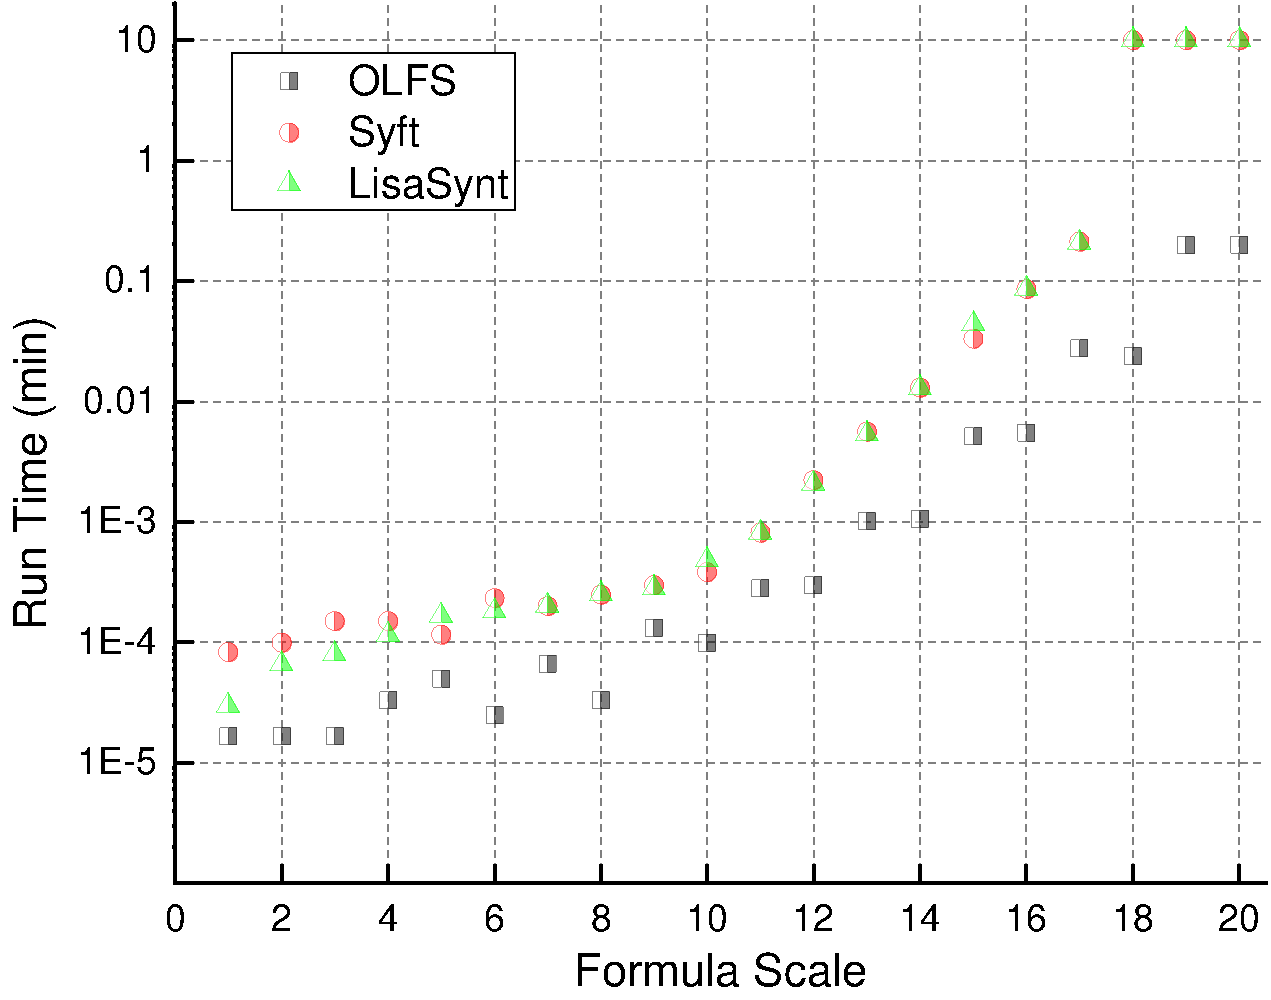
\includegraphics[width=5.5cm]{pic1_1.pdf}
    \caption{Results on the pattern formula $U (n) = p_1\U(p_2\U(...\U p_n))$.}
    \label{fig:preprocess-1}
\end{minipage}%
% }%
% \subfigure{
\begin{minipage}{0.33\linewidth}
\centering
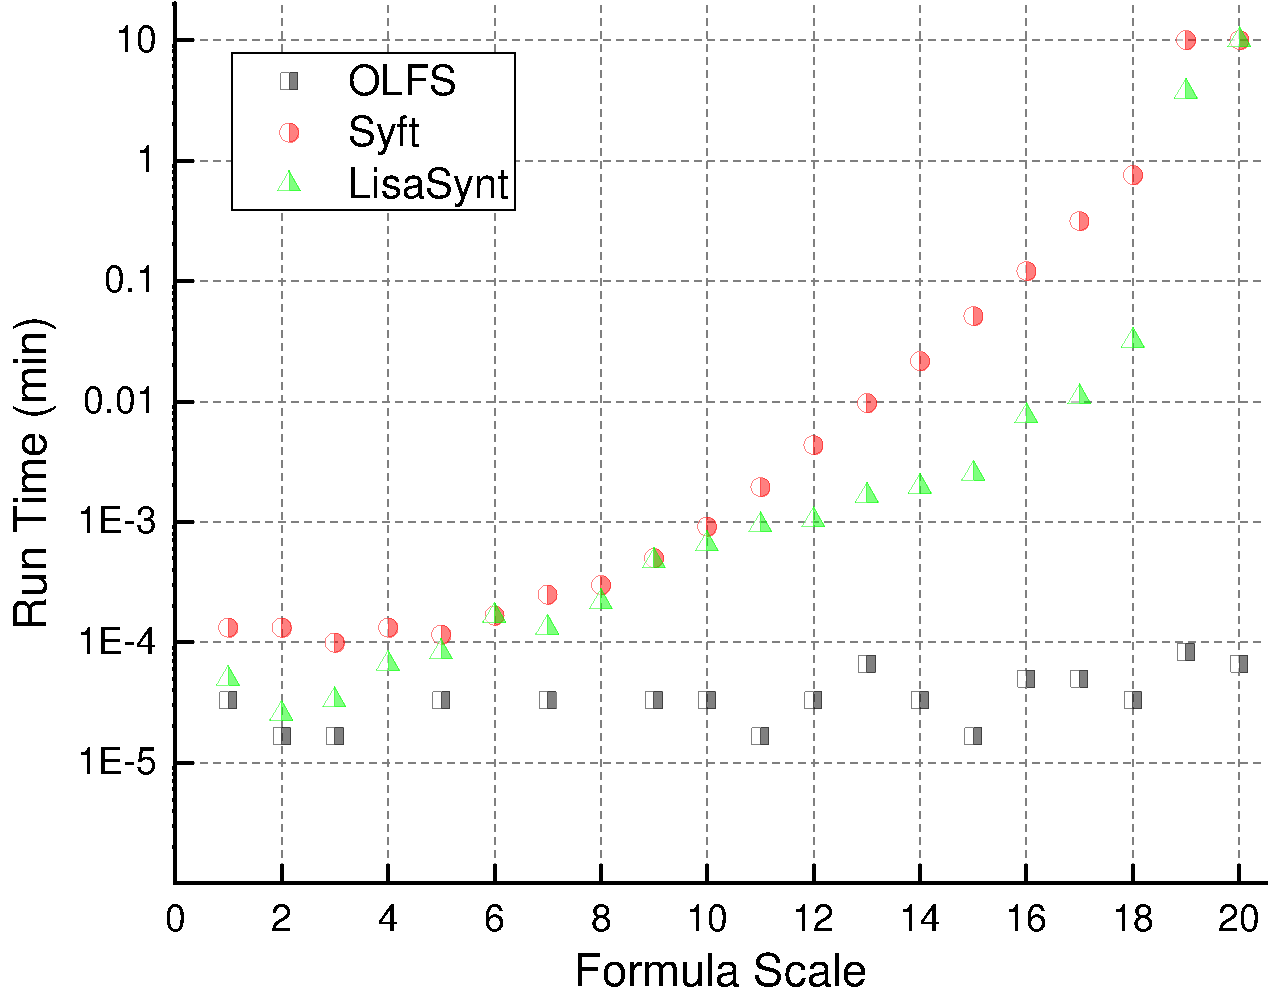
\includegraphics[width=5.5cm]{pic1_2.pdf}
    \caption{Results on the pattern formula $GF (n) = \G p_1\wedge(\bigwedge_{i=2\cdots n}\F p_i)$.}
    \label{fig:preprocess-2}
\end{minipage}%
% }%
% \subfigure{
\begin{minipage}{0.33\linewidth}
\centering
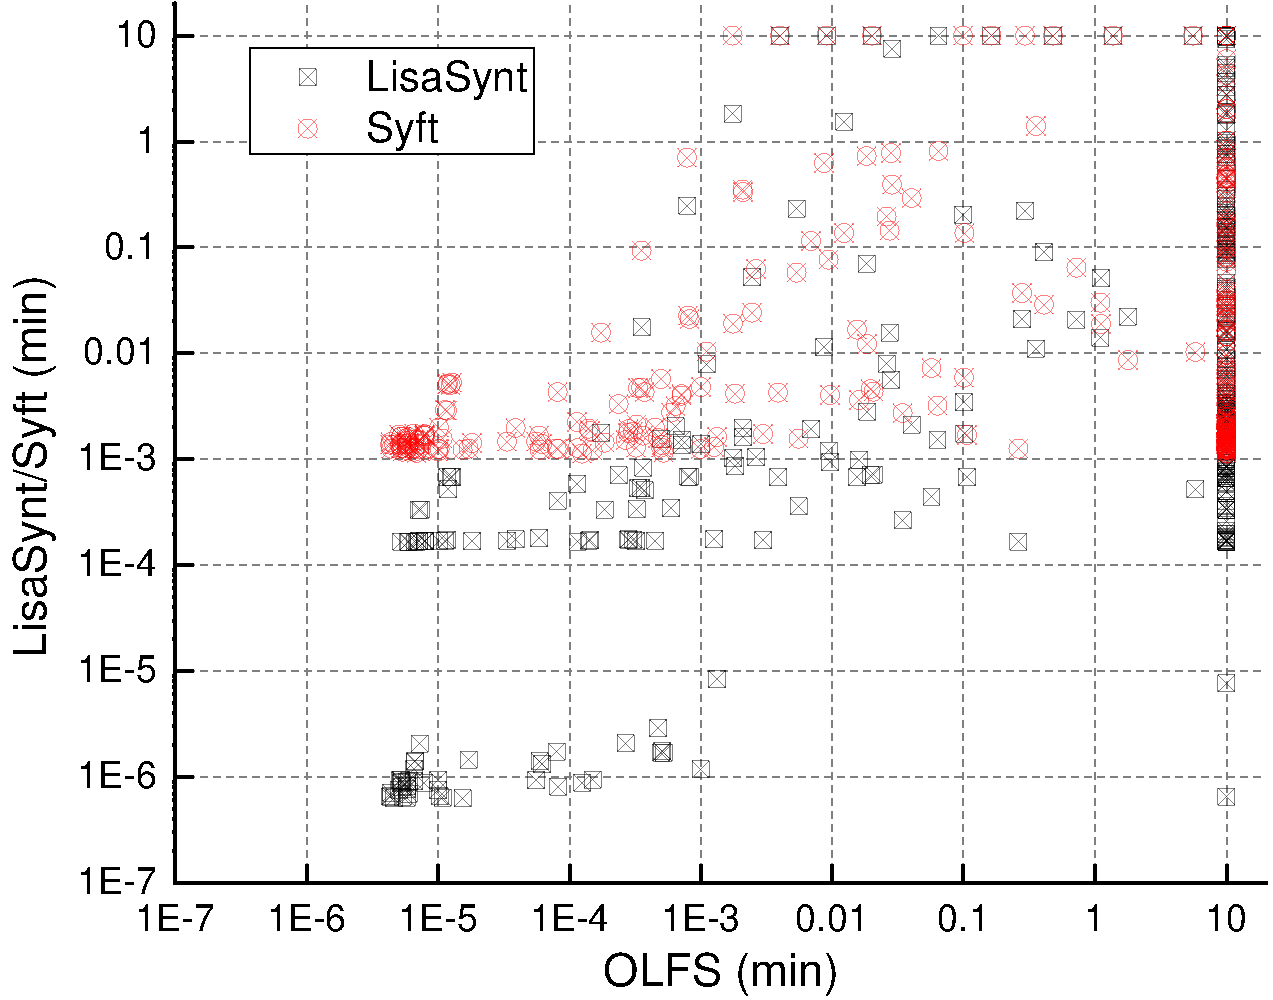
\includegraphics[width=5.5cm]{pic2.pdf}
    \caption{Results on the benchmarks from~\cite{BLTV20}.}
        \label{fig:otf}
\end{minipage}
% }%
\end{figure*}

Let $\Omega = \tool (\phi, \X, \Y)$ and we now define the strategy generator based on $\Omega$. Notably, our strategy generator only returns one winning strategy due to the on-the-fly construction, while the approach in \cite{GV15} is able to return all possible winning strategies. 

\begin{definition}[Strategy Generator]\label{def:transducer}
	The strategy generator for the \ltlf synthesis problem $(\phi, \X, \Y)$ is a transducer $\mathcal{T}_{\A}=(2^{\X\times\Y}, S, s_0, \xi, \sigma)$ such that
	\begin{itemize}
		\item $2^{\X\times\Y}$ is the alphabet of the transducer;
		\item $S = \{s| \langle s, Y, \{\langle X, s'\rangle\}\rangle \in\Omega\}\subseteq 2^{2^{\cl(\phi)}}$ is the set of states;
		\item $s_0 = \{\{\phi\}\}$ is the initial state;
		\item $\xi: S\times 2^{\X}\rightarrow 2^S$ is the transition function such that $\xi (s, X) = \{s' | \langle s, Y, \{\langle X, s'\rangle\}\rangle\in \Omega\}$;
		\item $\sigma: S\rightarrow 2^{\Y}$ is the output function such that $\sigma(s)=\{Y | \langle s, Y, \{\langle X, s'\rangle\}\rangle \in \Omega\}$.
	\end{itemize}
\end{definition}






